%% Except where otherwise noted, content in this documentation is Copyright (c)
%% 2015-2019, RTE (http://www.rte-france.com) and licensed under a
%% CC-BY-4.0 (https://creativecommons.org/licenses/by/4.0/)
%% license. All rights reserved.

\documentclass[a4paper, 12pt]{report}

% Latex setup
%%  Copyright (c) 2015-2019, RTE (http://www.rte-france.com)
%%  See AUTHORS.txt
%%  All rights reserved.
%%  This Source Code Form is subject to the terms of the Mozilla Public
%%  License, v. 2.0. If a copy of the MPL was not distributed with this
%%  file, you can obtain one at http://mozilla.org/MPL/2.0/.
%%  SPDX-License-Identifier: MPL-2.0
%%
%%  This file is part of Dynawo, an hybrid C++/Modelica open source time domain
%%  simulation tool for power systems.


%%%%%%%%%%%%%%%%%%%%%%%%%%%%%%%%%%%%%%%%%%%
% Define text and document settings
%%%%%%%%%%%%%%%%%%%%%%%%%%%%%%%%%%%%%%%%%%%

\usepackage{lmodern} % Latin Modern fam­ily of fonts
\usepackage[english]{babel} % English

% Specify encoding
\usepackage[utf8]{inputenc} % Input
\usepackage[T1]{fontenc} % Output

% Document structure setup
\usepackage{titlesec} % To change chapter format
\setcounter{tocdepth}{3} % Add subsubsection in Content
\setcounter{secnumdepth}{3} % Add numbering for subsubsection
\setlength{\parindent}{0pt} % No paragraph indentation

% Avoid numbering starting at each chapter for figures
\usepackage{chngcntr}
\counterwithout{figure}{chapter}

% Change title format for chapter
\titleformat{\chapter}{\Huge\bf}{\thechapter}{20pt}{\Huge\bf}

% To add links on page number in Content and hide red rectangle on links
\usepackage[hidelinks, linktoc=all]{hyperref}
\usepackage[nottoc]{tocbibind} % To add biblio in table of content
\usepackage{textcomp} % For single quote
\usepackage{url} % Allow linebreaks in \url command
\usepackage{listings} % To add code samples

% Define typography
\usepackage{xspace}
\usepackage{dirtree}
\newcommand{\Dynawo}[0]{Dyna$\omega$o\xspace}

% Default listings parameters
\lstset
{
  aboveskip={1\baselineskip}, % A bit of space above
  backgroundcolor=\color{shadecolor}, % Choose the background color
  basicstyle={\ttfamily\footnotesize}, % Use font and smaller size \small \footnotesize
  breakatwhitespace=true, % Sets if automatic breaks should only happen at whitespace
  breaklines=true, % Sets automatic line breaking
  columns=fixed, % Nice spacing -> fixed / flexible
  mathescape=false, % Escape to latex false
  numbers=left, % Where to put the line-numbers
  numberstyle=\tiny\color{gray}, % The style that is used for the line-numbers
  showstringspaces=false, % Do not emphasize spaces in strings
  tabsize=4, % Number of spaces of a TAB
  texcl=false, % Activates or deactivates LaTeX comment lines
  upquote=true % Upright quotes
}

%%%%%%%%%%%%%%%%%%%%%%%%%%%%%%%%%%%%%%%%%%%
% Define plots settings
%%%%%%%%%%%%%%%%%%%%%%%%%%%%%%%%%%%%%%%%%%%

% Macro pack­age for cre­at­ing graph­ics
\usepackage{tikz}
\usepackage{subfigure}
\usepackage{float}

% Draws func­tion plots (based on pgf/tikz)
\usepackage{pgfplots}
\pgfplotsset{enlarge x limits=false, xlabel={\begin{small}$time$ (s)\end{small}}, height=0.6\textwidth, width=1\textwidth}
\pgfplotstableset{col sep=semicolon}

% Define colors
\usepackage{color}
\definecolor{blue}{rgb}{.3,.5,1}
\definecolor{deepblue}{rgb}{0,0,1}
\definecolor{darkblue}{rgb}{0,0,.4}
\definecolor{red}{rgb}{1,0,0}
\definecolor{darkred}{rgb}{.56,0,0}
\definecolor{pink}{rgb}{.933,0,.933}
\definecolor{purple}{rgb}{0.58,0,0.82}
\definecolor{green}{rgb}{0.133,0.545,0.133}
\definecolor{darkgreen}{rgb}{0,.4,0}
\definecolor{gray}{rgb}{.3,.3,.3}
\definecolor{darkgray}{rgb}{.2,.2,.2}
\definecolor{shadecolor}{gray}{0.925}

%%%%%%%%%%%%%%%%%%%%%%%%%%%%%%%%%%%%%%%%%%%
% Define blocks for simple network drawings
%%%%%%%%%%%%%%%%%%%%%%%%%%%%%%%%%%%%%%%%%%%

% Define blocks for newtorks drawings
\usepackage{amsmath} % Add math­e­mat­i­cal fea­tures
\usepackage{schemabloc} % Add block diagram library (french one)

%% Define infinite bus
\tikzset{infinite bus/.pic={
  code={
  \draw (0,0) circle (2) node[inner sep=0, outer sep=0] {{$\infty$}};
  \draw (2,0) --++ (2,0);
  }
  }
}

%% Define transformer
\tikzset{transfo/.pic={
  code={
  \draw (0,0) circle (2);
  \draw (2,0) circle (2);
  \draw (4,0) --++ (4,0);
  \draw (-2,0) --++ (-4,0);
  }
  }
}

%% Define generator
\tikzset{generator/.pic={
  code={
    \draw (0,0) circle (2);
    \draw (0,0) arc (0:180:0.5);
    \draw (0,0) arc (180:360:0.5);
    \draw (-2,0) --++ (-2,0);
  }
  }
}

%% Define generator controls
\tikzset{VR/.pic={
  code={
  \draw (0,0) circle (2) node[inner sep=0, outer sep=0] {{VR}};
  }
  }
}

%% Define SVarC
\tikzset{SVarC/.pic={
  code={
  \draw (0,0) circle (4) node[inner sep=0, outer sep=0] {{SVarC}};
  }
  }
}


\begin{document}

\title{\Dynawo Functional Documentation}
\date\today

\maketitle
\tableofcontents

\chapter{Functional documentation}

\section[Dynawo Overview]{\Dynawo Overview}

The nature of power system dynamics is deeply evolving towards a more diverse and difficult to predict behaviour due to the massive changes going on in the power system (large penetration of power-electronic based components such as Renewable Energies Sources - RES - or High Voltage Direct Current - HVDC - lines, booming use of complex automata, control strategies or smart grids). Due to this radical change from physically-driven to numerically-driven dynamics, being able to assess the system stability becomes harder but is still essential as any generalized incident will be unacceptable for the economy and the consumers. This requires to have access to a transparent, flexible, robust and easy to use suite of simulation tools that will allow to run collaborative studies in a very simple way by sharing not only the same data but also the same modelling and solving choices in an open-source frame. Such a suite of simulation tools will ensure to get similar results and to agree upon optimal and shared actions on the system to accompany the ongoing changes in the best possible way. This analysis has motivated us to launch a new effort on simulation tools that finally ends up in the development of the \Dynawo's initiative. \\

\textbf{To achieve this goal, \Dynawo is based on two mains principles: the use of a high-level modelling language \href{https://modelica.org/} {\underline{Modelica}} and a strict separation between modelling and solving parts}.\\

\begin{figure}[h!]
\centering
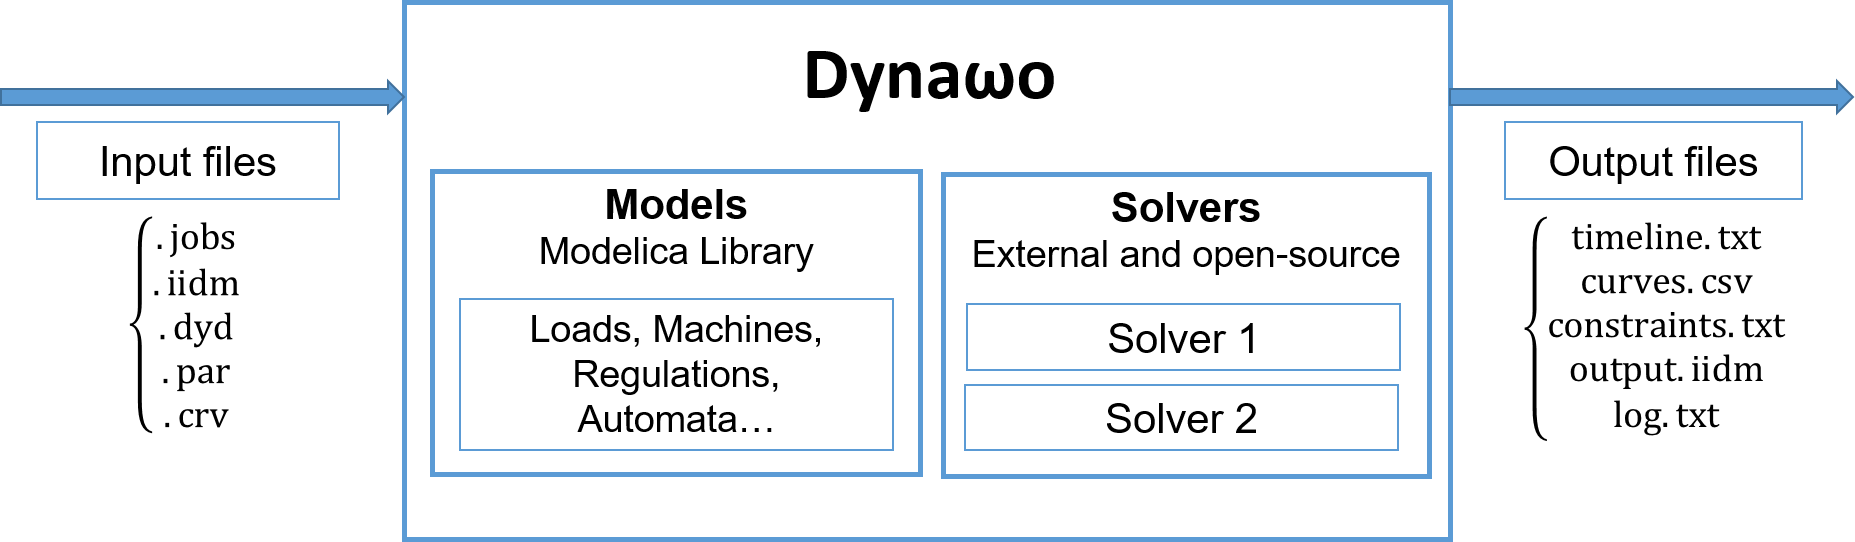
\includegraphics[width=\textwidth]{../resources/DynawoModelSolver.png}
\caption{Separation between modelling and solving parts in \Dynawo}
\end{figure}

\textbf{Modelica is an equation-based, declarative and object-oriented modelling language that is easy to read and understand}. The equations are written in a similar way as how they are written in textbooks for example. Using this language enables to easily share and discuss the modelling choices done because the final models implementation is available in an understandable way, even for the end-user. The Modelica language is already used in different and various industrial sectors. It is important to mention that Modelica-based tools already exist (Dymola, OpenModelica, JModelica, etc.) but they are not efficient enough for large-scale simulation of power system, which was one of the motivation for developing \Dynawo. In addition to this, the Modelica language itself has some limitations that are addressed in \Dynawo by the possibility to use C++ models in a similar way as Modelica models. Anyway, in the end all Modelica models are converted to C++ by \Dynawo. \\

\textbf{In order to transform the Modelica code into an executable C code, \Dynawo uses \href{https://www.openmodelica.org/}{\underline{OpenModelica}}, which is an open-source Modelica-based modelling and simulation environment, and particularly the OpenModelica compiler}. OpenModelica is the Modelica open source environment that is the most widely used today in the Modelica community and that covers the best the language norm. As such and in order not to develop an in-house solution that will be difficult to maintain in the long-term, as well as to benefit from developments and progresses made for other industrial sectors simulations, we have made the choice to build \Dynawo upon OpenModelica. In addition to the transformation done by the OpenModelica compiler, Python scripts are implemented into \Dynawo to transform the outputs from the OpenModelica compiler in a generic frame that is also common to the C++ models available in \Dynawo. All the thereby generated C++ models are then combined to build a global model that will interact with the solving part.

\begin{figure}[h!]
\centering
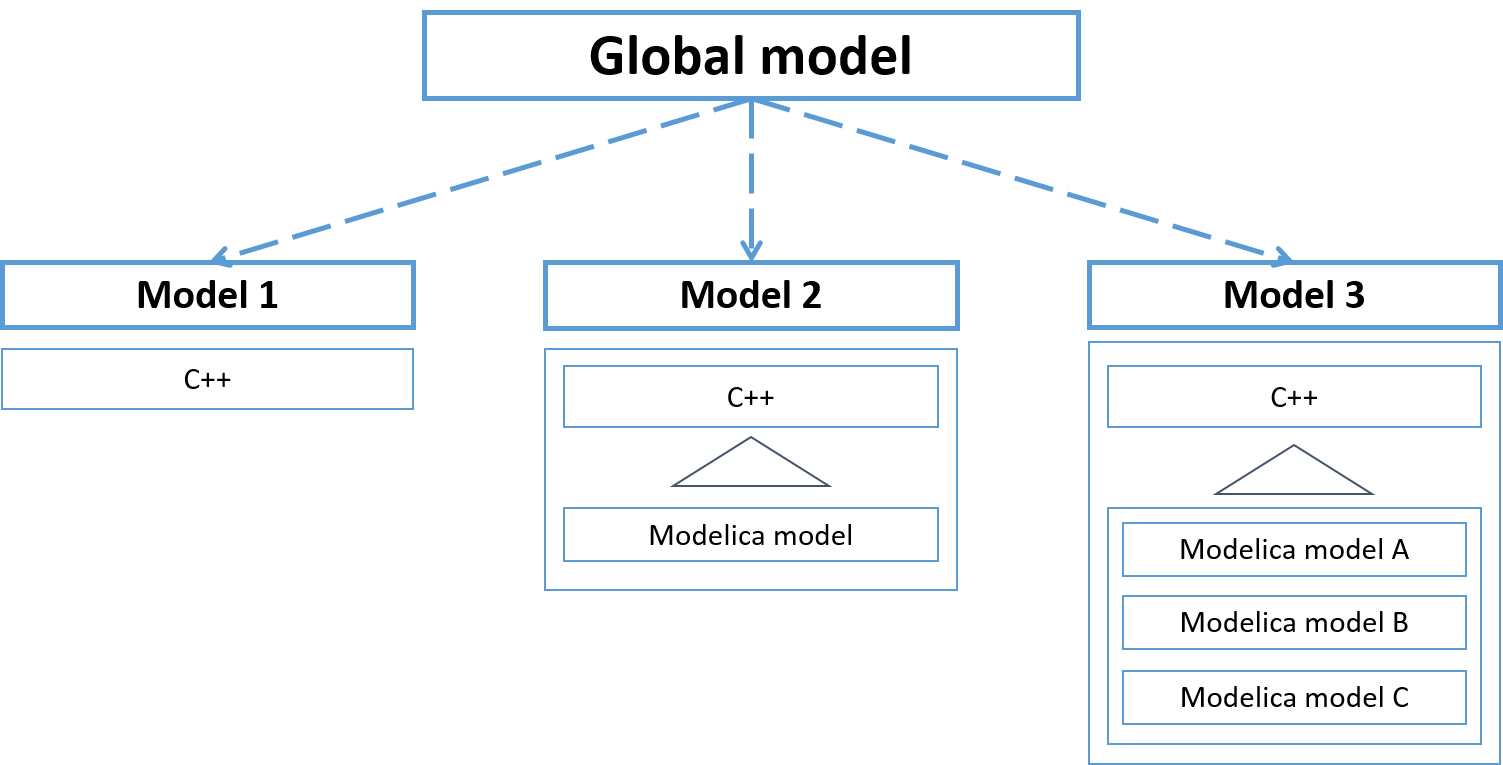
\includegraphics[width=\textwidth]{../resources/GlobalModel.png}
\caption{Building a global model from different unit models in \Dynawo}
\end{figure}

To ensure acceptable performances both for compilation and simulation, a mechanism has been created into \Dynawo to compile non squared Modelica models individually (for example a generator model by itself) and before the simulation. These compiled models are then only instantiated during the simulation. This strategy enables to use \Dynawo for large-scale simulations (French EHV-HV networks, in the range of 100 000 continuous variables and 150 000 discrete variables after simplifications) while keeping computation time in a range close to current simulation tools.\\

\textbf{The global model only exposes a few methods to the solvers} such as the residual functions, the Jacobian function or the zero-crossing functions. Having a separation between the modelling and the solving parts means that the choice of the numerical resolution method doesn't interfere with the models implementation. This feature has several advantages: it enables to easily test or use new solvers, it eases the addition of new model and it allows modelling experts not to bother about numerical difficulties and vice versa.

\begin{figure}[h!]
\centering
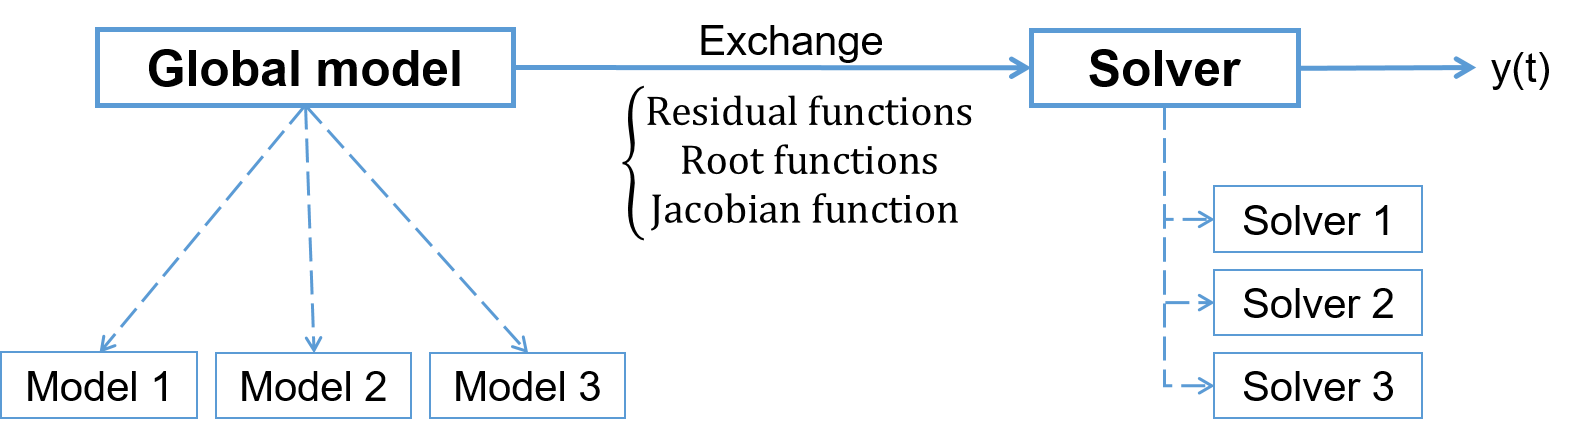
\includegraphics[width=\textwidth]{../resources/ExchangeModelSolver.png}
\caption{Exchange between the modelling and the solving parts in \Dynawo}
\end{figure}

\textbf{There are different solvers included into \Dynawo}:

\begin{itemize}
\item A fixed time-step solver developed for long-term stability studies that is based on works done during the European project \href{http://www.fp7-pegase.com/}{\underline{Pegase}}. It is a \ac{BE} solver that focuses more on performances than on accuracy as there is no control error scheme and events are detected and applied in a synchronous way at time instants corresponding to the time step values;
\item Another fixed time-step solver with similar properties than the first one but using a trapezoidal method instead of a \ac{BE} method for the numerical integration.
\item A variable time-step variable order BDF solver called IDA and developed by the Lawrence Livermore National Lab as part of the \href{https://computation.llnl.gov/projects/sundials}{\underline{SUNDIALS}} suite of solvers. Contrary to the first solver, IDA aims at running very accurate simulations by using a control error scheme and by detecting the exact instant corresponding to an event, thanks to its root findings mechanism.
\end{itemize}

One important idea in \Dynawo is that the same models could be used for different stability studies. It is the overall association between the different models and the selected solving strategy that enables to run a specific stability study. For example, short-term stability studies and long-term stability studies share a large common set of models but use different solving strategies. Indeed, short-term stability studies are simulated using the \ac{IDA} solver which manages to capture the fast dynamics while long-term stability studies are done with the simplified solver that approximates the fast dynamics but enables to study the system long-term behavior with very good simulation times.  \\

\Dynawo 's primary focus has been on long-term and short-term stability studies but the very encouraging results obtained and the flexibility of the approach led to an extension of the initiative. \textbf{\Dynawo is now evolving towards a complete and coherent suite of simulation tools}, sharing the same philosophy:
\begin{itemize}
\item DynaFlow for steady-state calculations
\item DySym for short-circuit calculations
\item DynaWaltz for long-term stability simulations
\item DynaSwing for short-term stability studies
\item DynaWave for stability studies and system design with a high-penetration of power-electronics based components (quasi-EMT)
\end{itemize}

\begin{figure}[H]

\includegraphics[width=\textwidth]{../resources/DynawoLogos.png}
\end{figure}

\begin{figure}[H]
\centering
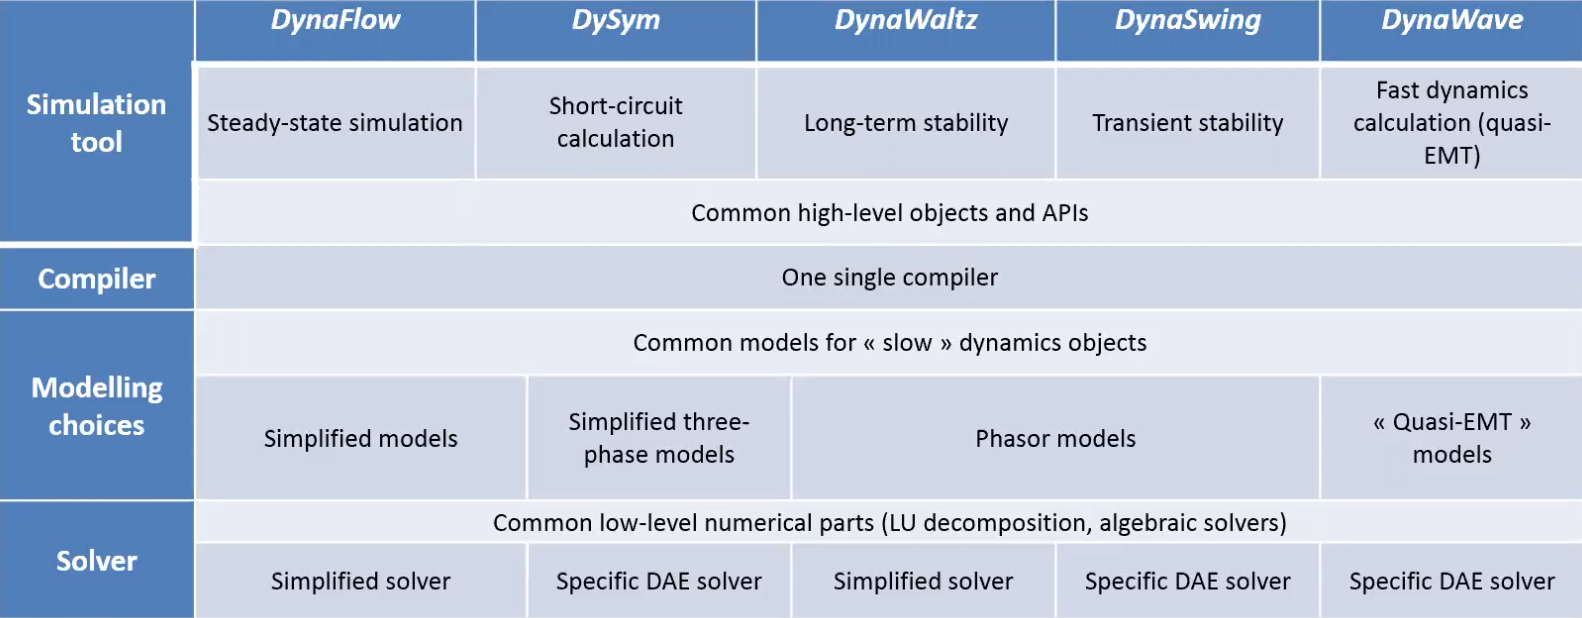
\includegraphics[width=\textwidth]{../resources/DynawoInitiative.png}
\caption{High-level vision of the \Dynawo initiative}
\end{figure}

More details on the philosophy of \Dynawo could be found into \cite{Dynawo}.

\newpage
\subsection{DynaFlow}

\textbf{One important and fundamental simulation tool for real-time operation and planning studies of the power system is the steady-state calculation tool.} This tool focuses on the correct calculation of the system equilibrium point following one or several event(s): it ensures the existence of a steady-state point and enables to check that this point is acceptable for the system operator. \\

This calculation has been historically done by \textit{purely static simulation tool} determining the final steady state by the combination of outer heuristic loops - trying to mimic the actions of special protection schemes, controllers and regulations - and an inner loop - classical power flow problem - solved several times. The recent and ongoing power system evolution - power-electronics based components, diverse and advanced controllers, etc. - makes this classical approach null and void for modern power system steady-state calculations. \textbf{Indeed, the steady-state point is determined by the difference of speeds of the various controls, regulations and special protection schemes dynamics}. It is thus absolutely necessary to represent the actions temporality to find the correct steady-state point and takes the best decisions when operating the system or planning new investments for the future. \\

\textbf{DynaFlow is a new steady-state simulation tool that aims at calculating the steady-state point by using a simplified time-domain simulation, guaranteeing the correctness of the solution found.} The \textit{Illustrative Test Cases} example section as well as the \textit{IEEE14 and WSCC9 test cases} show the pros of this approach compared to a purely static simulation tool. Preliminary studies on the French-Spain border have proved the advantages of the approach over classical static simulation tool, allowing to have an higher maximum flow accross the border in realistic situations.\\

The modeling approach chosen for DynaFlow is available into the following publication \cite{DynaFlow}.
Regarding performances, DynaFlow exhibits similar performances than classical steady-state simulation tools for the simulation part (core part) and improvements on the initialization part are scheduled in the next few months to further reduce the cost of input/output on the simulation time. \\

In order to ease the creation of input data and the usability of DynaFlow, a separate project called DynaFlow-launcher (\url{https://github.com/dynawo/dynaflow-launcher}). It enables to create all the necessary files from a single iidm file, based on predefinite rules for each component.

\begin{center}

\includegraphics[width=0.3\textwidth]{../resources/DynaFlow.png}
\end{center}

\newpage
\subsection{DySym}

\textbf{Short-circuit calculations are essential simulations for power system operators.} They are used to avoid large incidents on the system during its operation but also to avoid reaching situations that can damage materials, the environment or even injure people. \\

Until the recent years, the power system short-circuit behavior was mainly driven by the synchronous machines actions and the interesting result was obtained for the transient part following the event (around $100 \ ms$ after the event). Considering this, it was adequate enough to do one static calculation with a specific machine representation ($E$ behind $X_{d}$) to analyze potential short-circuit issues. Nevertheless, the large introduction of power-electronics based components that can have very different behaviors, mainly defined by the tuning of their controls, deeply modify the system behavior during a short-circuit. \textbf{Short-circuit calculations have to evolve to accurately take into account the power-electronics based components participation during the fault.} \\

\textbf{Our ambition with DySym is to provide a short-circuit simulation tool that is adapted to the current and future power system operators needs.} Through a time-domain approach correctly representing the different power system components and their contribution during the short-circuit, the user will have the possibility to output different values to further analyze the system behavior. \\

\textbf{DySym is at a research stage and we are currently playing around with different models to see which hypothesis make sense and which modelling choices should be done.} We plan to release a work plan as soon as possible and then distribute a first proof of concept. Don't hesitate to have a look to our website to see the current status.

\begin{center}

\includegraphics[width=0.3\textwidth]{../resources/DySym.png}
\end{center}

\newpage
\subsection{DynaWaltz}

\textbf{Long-term stability studies are a core process for ensuring power system stability: they enable to guarantee that the slow dynamics of the system don't lead to an instability or a system collapse}.\\

Most of the classical approaches for long-term stability studies use simplified models to reach acceptable simulation times on large-scale systems. The quasi steady-state simulation approach is the most widely known approximation: it consists in considering the fast dynamics stabilized and thus in replacing their differential nature by pure algebraic equations (for example, an integral control for voltage regulation can be considered instantaneous). While this technique globally provides acceptable results on most of the situations, \textbf{it involves a strong a priori hypothesis on the real system behavior}. This approximation is more and more questionable in a system where the multiplicity and diversity of the controls is exploding. \\

\textbf{Our long-term stability simulation tool DynaWaltz uses a different paradigm. Instead of doing a priori simplifications or hypothesis on the modelling side, it is the numerical method that will take charge of filtering the fast dynamics while keeping as detailed models as necessary.} Thanks to an intensive research work conducted during the Pegase project on the numerical method and an important effort on the simulation tool itself (\cite{SpeedUpDynaWaltz}), DynaWaltz manages to achieve simular simulation times than current long-term stability simulation tools.\\

\textbf{DynaWaltz is the most advanced simulation tool of the \Dynawo initiative. It is operationnaly used on a daily basis in RTE national control center to deal with voltage stability issues.} In its operational use, DynaWaltz enables to launch individual simulation but also contingency analysis as well as  margin calculation thanks to the algorithms implemented and available into the dynawo-algorithm repository (\url{https://github.com/dynawo/dynawo-algorithms}).

\begin{center}

\includegraphics[width=0.2\textwidth]{../resources/DynaWaltz.png}
\end{center}

\newpage
\subsection{DynaSwing}

\textbf{In order to protect the system against loss of synchronism or inter-area oscillations, the system operator has to conduct a large number of short-term stability studies. }Transient stability focuses on phenomena in the range of the ms and depends mainly on the active component models - synchronous machines and their controllers, HVDCs, Static Var Compensators. \\

To properly represent the system response in the few instants following an event, \textbf{it is necessary to combine open models with detailed physical modelling and transparent block control scheme with a very accurate solving method.} It is the association of these different features that enable to catch the correct system fast dynamics. \\

\textbf{DynaSwing is a simulation tool that offers an unique combination of a transparent, flexible and robust way of modelling - thanks to the intensive use of the Modelica language - and a state-of-the-art, efficient and accurate numerical method (the variable time-step solver IDA).} \\

\textbf{The core of the tool has already reached a mature state, making it usable for running transient stability studies.} The future work will thus concentrate on:
\begin{itemize}
\item the development of more elaborated regulation controls (PSS, specific governors or voltage regulators)
\item the addition of new models (especially standard PV and wind models)
\item the improvement of the numerical method on large test cases (especially on systems containing a lot of digital controllers).
\end{itemize}
These developments will contribute to enlarge the possibilities offered by DynaSwing.

\begin{center}
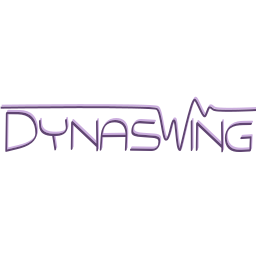
\includegraphics[width=0.3\textwidth]{../resources/DynaSwing.png}
\end{center}

\newpage
\subsection{DynaWave}

\textbf{Being able to correctly design the future system and to anticipate the needed changes in grid codes and system regulations is critical to be able to operate the grid in the future.} Indeed, the overall energy sector is going through a major evolution powered by a general will for \textit{clean energy} that ends up in a move towards a larger development and integration of renewable energies sources in the power system. \\

\textbf{The traditional stability boundaries are challenged by this global change.} In a system with a high percentage of power electronics based components, the classical \textit{phasor approach} may be unadapted and unable to capture all the possible interactions between the different controllers themselves and between the controllers and the system, leading to inappropriate control and regulations designs that can end up in future large incidents on the system. \\

The aim of DynaWave is to propose a new simulation frame to correctly capture fast dynamics phenomena occuring in systems with a high penetration of renewable energy sources. \textbf{The modeling frame chosen would consist in a \textit{quasi-EMT} approach, being more detailed than the phasor approach without encompassing the complexity of an EMT simulation.} \\

The development and release of some grid-forming controllers strategies and of dynamic lines are the first steps on which DynaWave will be built. They allow to simulate in a completely open-source environment the three nodes test case used in the Migrate project to study interactions between different grid-forming controllers (the test case is under final validation but will be released soon). \textbf{The idea is to build upon this first basis to develop more open-source models, in collaboration with our partners and colleagues conducting researches on stability of power systems with a high-share of power-electronics based components.} DynaWave will provide a flexible and open-source simulation tool to ease technical discussions and collaborations in order to face the future stability challenges arising in power-electronics based system.

\begin{center}

\includegraphics[width=0.18\textwidth]{../resources/DynaWave.png}
\end{center}

\newpage
\section{Models}

\subsection{Introduction}

\Dynawo\textquotesingle s library is divided into two parts: a C++ part and a Modelica part. \\

Modelica is the favourite modelling language in \Dynawo for a lot of different reasons: it is an open source language, widely used in different industrial sectors (automotive, building, etc.), that is equation-based, declarative, high-level and object oriented. It means that the person in charge of the modelling task doesn't have to bother about the way the equations will be solved but only on the necessity to have as many equations as variables, which makes it possible to just use equations from reference papers or textbooks without having to modify them. With such an approach, model sharing becomes a reality in the sense that it is very easy for any user to understand what is done in a model without having to spend a lot of time and energy in trying to understand the written code (as it is often the case with Fortran or C for example). Another advantage in a long-term perspective is the possibility to easily do multi-system simulations with a Modelica-based simulation tool. Indeed, by nature, Modelica is not specific to one domain and so it is possible (and some libraries already exist) to model prime movers or gas systems in Modelica. All these advantages have motivated the choice to use Modelica in \Dynawo. Nevertheless, the Modelica language also has a few drawbacks that prevent us to exclusively base our solution on Modelica. For example, it is very impractical to deal with connectivity analysis with Modelica models (which is required in power system simulations to deal with system splitting) or to have variable-size objects (there is no vector object in Modelica). \\

In order to be able to model any kind of object and to bypass the aforementioned Modelica\textquotesingle s limitations, it is possible to use C++ models in \Dynawo. This is particularly useful to model large-scale regulations that need to be connected to a large number of components or to deal with the network topology. \\

All library models are available in the ddb (dynamic database) repository generated by \Dynawo compilation and can be directly used into test cases. In addition, the ddb directory also contains the .so library corresponding to the preassembled models and two xml files - one describing the connection needed by the model *.xml and one describing the parameters required and the model variables *.desc.xml.  \\

Below is an example of a Pi line model in Modelica. As explained earlier, the model is easy to read and understand:

\lstinputlisting[language=Modelica,title=Pi Line implementation in Modelica]{../resources/Line.mo}

\subsection{C++ library}

The C++ library contains:
\begin{itemize}
\item A Components (\ref{Components}) directory that will contain all components implemented into C++ with a specific behavior not encompassed into the default C++ network model.
\item Events (\ref{Events}), and in particular a variation area model that applies a variation on the (P, Q) values of one area\textquotesingle s loads and a voltage set point change model sending a set point variation order to any other system component.
\item An explicit  frequency model (OmegaRef model) that calculates the rotation speed reference value for the system.
\item A network model (\ref{Network}) that provides a default behaviour for any grid component
\end{itemize}

\subsubsection{Components}
\label{Components}

A restorative load model with limits has been added to the C++ library. It can be used to represent in a continuous way the behavior of a load behind transformers equipped with tap-changers.

\subsubsection{Events}
\label{Events}

Two events are currently available in C++ models.

\paragraph{Variation area model}
~~\\

This model enables to calculate the active and reactive power variation to apply to a set of loads to match a given variation in a time window. Its parameters are thus the starting and stopping time of the variation and the required changes into P and Q.

\paragraph{Voltage set point change model}
~~\\

It allows to send a voltage set point change order to any other component of the system. The set point variation is sent during a time window and its value is a parameter of the model as well as the start and stop time of the variation.

\subsubsection{Frequency models}
\label{Frequency}

Two different frequency models are available into \Dynawo. When doing a simulation, an user has to either choose the explicit frequency model (OmegaRef) and the associated machine models or an implicit frequency model (SignalN) and the associated models. Only the explicit model is done in C++, the implicit one is implemented directly into Modelica.

\paragraph{Explicit frequency model - OmegaRef}
~~\\

The ``OmegaRef'' model calculates the reference speed for each synchronous area. This reference speed is determined by calculating a weighted barycentre of the different speeds of the generators connected to the grid in the synchronous area:

\begin{equation}
\begin{aligned}
& \omega_{ref} = \frac{\sum\limits_{i} H_i * S_{Nom, i} * \omega_{i}}{\sum\limits_{i} H_i * S_{Nom, i}}
\end{aligned}
\label{Speed reference calculation}
\end{equation}

This model is connected to all the generators of one synchronous area and takes their speed as inputs to calculate the reference speed that is used into the machine models.

\subsubsection{Network model}
\label{Network}

The C++ network model is fundamental in \Dynawo. Indeed, as soon as there is a static description of the network (iidm file) given in input, it is necessary to map a default behaviour to any component that can be present into the grid. Therefore, for each static component, there is a corresponding default behaviour into the network model. These models are used if and only if no other dynamic model is associated to the static component. Such a scheme ensures to be able to run simulations even without any dynamic data (or Modelica model). In this case, the simulation only uses the default C++ models. For most of these default models, the choice has been made to keep a very simple behaviour consisting in maintaining the original power flows and power injections (calculated a priori by a load flow module for example). \\
Each component is described with more details in the next parts. \\

\paragraph{Bus}
~~\\

The bus model contains two equations corresponding to the Kirchoff's law on the current $\sum i = 0$. It is also possible to turn on or turn off a bus during a simulation by using events. \\
In addition to this, the voltage module and angle are available as outputs both in per unit, kV or degree for display as well as the bus connection state. The model also enables to define an upper and a lower constraint limit for the bus' voltage. If they are violated, a constraint is printed out into the output constraint file. \\

\paragraph{Line}
~~\\

The default line model in \Dynawo is a classical $\pi$ line model.

\begin{figure}[h!]
\centering
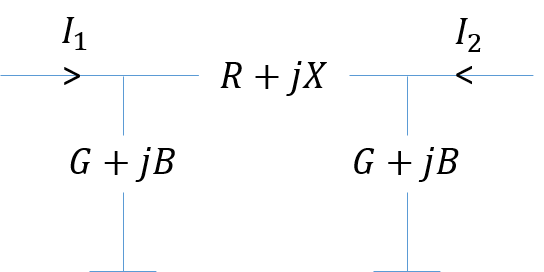
\includegraphics[width=60mm]{../resources/PiLine.png}
\caption{$\pi$ line model}
\end{figure}

The line can be connected or disconnected during the simulation, either on both sides or only on one side. In addition, the line model gives access to a large number of variables: P, Q or the current circulating into the line (at each side) and the line status (open/close/close on one side). \\
If such limits exist in the input file (iidm file), current maximum limits are added to the line. These limits correspond to the maximum current that the line can support during a certain time. If the line is overloaded during more time than this allowed time, the line will be tripped. \\

In addition, the line can also be dynamic. In this case, the derivative terms ($L * \frac{di}{dt}$ and $C * \frac{dv}{dt}$) are no longer neglegted. This model is available and can be activated by setting the following parameter $line\_isDynamic$ at true in the network set of parameters. Please notice anyway than the dynamic line model has not been as extensively used and validated as the other network components.

\paragraph{Transformer}
~~\\

Only two-windings transformers are handled by \Dynawo C++ model at the moment. In the transformer model, conductance and susceptance are only defined at the side 2 voltage level and they are, as the resistance and the reactance, defined in side 2 voltage per-unit basis. \\
The transformer model could be connected to either a phase shifter automaton to regulate the current on a line or to a tap changer to control the bus module voltage. The tap changer automaton modifies the voltage ratio applied between side 1 and side 2 to respect a certain set point on side 2, whereas the phase shifter can add a contribution to the voltage angle to change the power flow going through a line. There are logs indicating a tap change when the automata have to act. \\
As the line model it is possible to display the P, Q, current values going through the transformer. In a similar way, maximum current limits could be added to the transformer. \\

\paragraph{HVDC}
~~\\

The current implementation for the C++ HVDC model is a one that keeps P and Q on the HVDC AC sides constant. There is no calculation of any variables on the DC side. \\
The HVDC can be connected or disconnected during the simulation. The user can have access to the active and reactive power injected by the link on the network. \\

\paragraph{Generator}
~~\\

The generator model calculates the necessary current to follow set points for P and Q. It doesn't have any limits on P, Q or the current. The set points can be modified during the simulation and the generator can be connected or disconnected. In case the set point is modified, there is a log message displayed into the timeline output that indicates the set point new value(s). \\

\paragraph{Load}
~~\\

The load model can represent different behaviours, depending on the parameters given by the user. The generic equations defining the load behaviour are:

\begin{equation}
\begin{aligned}
& P = z_{P} * P_{0} * (1 + \Delta P_{C}) * (\frac{U}{U_{0}})^\alpha \\
& Q = z_{Q} * Q_{0} * (1 + \Delta Q_{C}) * (\frac{U}{U_{0}})^\alpha
\end{aligned}
\label{Load model}
\end{equation}

The possible behaviours are:
\begin{itemize}
\item A voltage dependant load if the load is neither declared as restorative or controllable - $z_{P} = z_{Q} = 1$ and $\Delta P_{C} = \Delta Q_{C} = 0 $. This is the default model.
\item A load with a possible variation coming from another model (for example the variation area model). In this case, there is a delta applied on P and Q at each instant that is determined by the other model. For example, if we choose to apply a variation of 10 MW over 10 s, the load value will vary by 1 MW every 1 s. In this case, $\Delta P_{C}$ and $\Delta Q_{C}$ are varying over time but $z_{P}$ and $z_{Q}$ are kept constant equal to 1. This is the controllable load model.
\item A restorative load model in which the load works as a first order restorative one. $z_{P}$ and $z_{Q}$ can vary during the simulation.
\end{itemize}

\begin{figure}[h]
  \setlength{\abovecaptionskip}{15pt}
  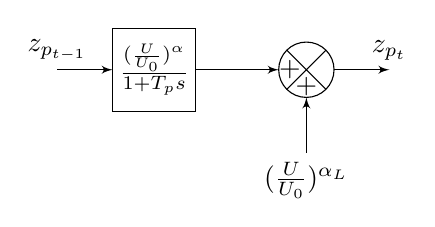
\begin{tikzpicture}[every node/.style={inner sep=0,outer sep=0}]
\sbEntree{E}
\sbStyleLien{node distance=1em}
\sbStyleBloc{inner xsep=2}
\sbBlocL{a}{$\frac{(\frac{U}{U_0})^\alpha}{1+T_p s}$}{E}
\sbNomLien[0.7]{E}{$z_{p_{t-1}}$}
\sbSumb{b}{a}
\sbRelier{a}{b}
\sbDecaleNoeudy[3]{b}{c}
\sbRelier{c}{b}
\sbNomLien[-1]{c}{$(\frac{U}{U_0})^{\alpha_L}$}
\sbSortie{S}{b}
\sbRelier{b}{S}
\sbNomLien[0.7]{S}{$z_{p_{t}}$}
\end{tikzpicture}
\centering
\caption{Restorative load model}
\end{figure}

Any load model can be connected or disconnected. It is also possible for the user to have access to the output $P$, $Q$,$ P_C$ and $Q_C$ values. \\

\paragraph{Shunt}
~~\\

The shunt provides a constant reactive injection to the network. It can be connected or disconnected either by an user action or by an automaton action. \\
In order to simulate the necessary time between two actions on the same shunt, a minimal waiting time has been introduced into the shunt model between two actions (parameter noReclosingDelay). \\

\paragraph{Static Var Compensator}
~~\\

The static var compensator model controls the susceptance to respect a predefine set point. This is done through a PI structure as shown in Figure \ref{StaticVarCompensator} control scheme:

\begin{figure}[h]
  \setlength{\abovecaptionskip}{15pt}
  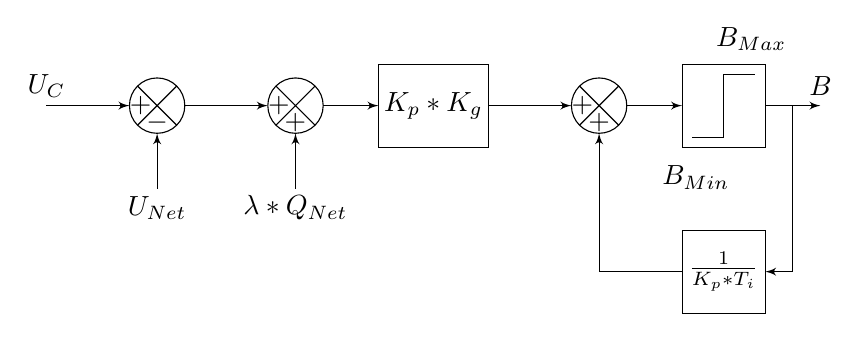
\begin{tikzpicture}[every node/.style={inner sep=0,outer sep=0}]
\sbEntree{E}
\sbStyleLien{node distance=1em}
\sbStyleBloc{inner xsep=2}
\sbComp{comp}{E}
\sbRelier{E}{comp}
\sbNomLien[0.7]{E}{$U_C$}
\sbDecaleNoeudy[3]{comp}{UNet}
\sbRelier{UNet}{comp}
\sbNomLien[-0.7]{UNet}{$U_{Net}$}
\sbSumb{addQ}{comp}
\sbRelier{comp}{addQ}
\sbDecaleNoeudy[3]{addQ}{Q}
\sbRelier{Q}{addQ}
\sbNomLien[-0.7]{Q}{$\lambda*Q_{Net}$}
\sbBlocL{GainKpKg}{$K_p * K_g$}{addQ}
\sbSumb{feedback}{GainKpKg}
\sbRelier{GainKpKg}{feedback}
\sbBlocL{Limiter}{\tikz {\draw (-0.4,-0.4) -- (0,-0.4);\draw (0,-0.4) -- (0,0.4); \draw (0,0.4) -- (0.4,0.4);)}}{feedback}
% Creating BMin
\sbDecaleNoeudy[3]{Limiter}{BMin}
\sbDecaleNoeudx[-1]{BMin}{BMinName}
\sbNomLien{BMinName}{$B_{Min}$}
% Creating BMax
\sbDecaleNoeudy[-2]{Limiter}{BMax}
\sbDecaleNoeudx[1]{BMax}{BMaxName}
\sbNomLien{BMaxName}{$B_{Max}$}
\sbSortie{S}{Limiter}
\sbRelier{Limiter}{S}
\sbNomLien[0.7]{S}{$B$}
\sbDecaleNoeudy[6]{S}{PINode}
\sbBlocr{PI}{$\frac{1}{K_p * T_i}$}{PINode}
\sbRelieryx{Limiter-S}{PI}
\sbRelierxy{PI}{feedback}
\end{tikzpicture}
\centering
 \caption{Static Var Compensator model}
 \label{StaticVarCompensator}
\end{figure}

\subsection{Modelica library}

The \Dynawo Modelica library contains several models to describe advanced dynamic behaviours of the main grid components as well as simple models equivalent to the C++ default models that are mainly used for testing in full Modelica simulations. \textbf{If the reader wants to have a look to the models, we highly recommend he/she to open the \Dynawo Modelica library with OpenModelica and in particular OMEdit: it provides a nice and rich environment to visualize the equations and the control blocks, as well as an immediate access to the library documentation and to some full Modelica test cases. } \\

In addition to the individual models (.mo files), \Dynawo\textquotesingle s code contains ``preassembled'' models that consist in a group of Modelica models that are compiled together to create a single final model library (.so) that could be directly used in the simulation (without being compiled at run time). These preassembled models correspond to a coherent dynamic behaviour (physical model + regulation models) and are built to be associated to one static component. One example is the combination of a synchronous machine model with its regulations (voltage regulators and governors). This gives one preassembled model that can be directly used during the simulation and associated to one particular generator (without having to associate the three models to the generator).

\subsubsection{Library content}

In this part, we will briefly describe what is the content of \Dynawo\textquotesingle s Modelica library. To understand in details the behaviour of each model and the chosen modelling assumptions, we encourage the reader to directly dig into the Modelica  model or to look at the specific documentation included into the model and available in a Modelica environment.\\

The \Dynawo library is divided into four main parts plus auxiliary packages (Types, AdditionalIcons and UsersGuide):
\begin{itemize}
\item The ``Connectors'' part contains all the specific connectors defined into \Dynawo that are used to connect together different models. This enables to have clear interfaces between the different models or the different parts of a model (regulation and physical model for example). For each type of variable, there is a type of connector (BPin for boolean values, ZPin for discrete values, ImPin for real values and ACPower for connecting both complex voltages and complex currents)
\item The ``Electrical'' part with the different models of the electrical components and their controls.
\item The ``Examples'' part with simple test cases to illustrate the way to use \Dynawo models in a full Modelica environment. Each test case has been configured with the best options available in OpenModelica for power sytem simulations.
\item The ``NonElectrical'' part including all \Dynawo - specific blocks. In the library, we have tried to use as much as possible existing blocks from the Modelica Standard Library but when necessary, specific models or blocks have been developed and are stored into this folder to be reused several times. This folder also contains logs files that are used to generate logs from the Modelica model during a simulation.
\end{itemize}

More details on the ``Electrical'' package are given in the next sections.

\paragraph{Buses}
~~\\

The bus package contains a simple Bus model and two versions of InfiniteBus model (a standard fixed one and an infinite bus model in which the voltage module and the frequency can vary). No other bus models are provided in the package as the default C++ model is generally used in \Dynawo simulations and is simple enough to be understandable by everyone, even written in C++.

\paragraph{Controls}
~~\\

The controls package gathers all the controls and regulations models for the different components:
\begin{itemize}
\item Common models, such as set point, perturbation, step and switch-off, are included into the Basics package.
\item The Converters package which features three types of grid forming controls. See \cite{GridForming} for more info.
\item The Current package includes a current limit automaton model and a phase shifter blocking I model (stopping the action of the phase shifter if the current becomes too high).
\item The Frequency package has the implicit frequency model, called SignalN.
\item The Generic package contains an example implementation to call a C function from a Modelica model. This model can serve for example to include an OPF-based automaton into a \Dynawo simulation.
\item The HVDC package contains two power transfer controls that enable one link to compensate the loss of another link in parallel.
\item The Machines package with the different regulations for the machines such as voltage regulations, governors, power system stabilizers or under-voltage protection. Regulations are then classified depending on their origin: simplified regulations, standard regulations, etc.
\item The \ac{PLL} package contains a \ac{PLL} model.
\item The Transformers package that includes the phase-shifter and tap changer automata models.
\item The Voltage package containing different tap changer blocking automata (depending on the number of voltages being monitored) and a remote voltage regulator model.
\item The \ac{WECC} package holds all the basic and final control structures associated to the \ac{WECC} components implemented into the \Dynawo library, in particular the wind and photovoltaics models.
\end{itemize}

\paragraph{Events}
~~\\

Events models enable to change the connection status of the different grid elements. They are all based on a similar basis with a time corresponding to the event and a variable whose value will change at the event time.

\paragraph{HVDC}
~~\\

The HVDC package contains different HVDC models: complete standard VSC model for long-term and short-term stability studies and simplified models:
\begin{itemize}
\item The HvdcPQProp models are simplified VSC models, with a proportional reactive control and a certain active power flowing into the link.
\item The HvdcPV models are simplified VSC models, that regulates the network voltage at both sides and respects a certain active power flowing into the link (represented as a constant loss factor).
\item The HvdcPTanPhi are simplified LCC models, for which the reactive power output is calculated thanks to a power factor and the active power is set (with constant losses in the DC line as for the HvdcPV model).
\item The HvdcVSC models are standard VSC models, with a complete control scheme (active power control, dc and ac voltage control, etc.) and a physical DC line model. More details are available in \cite{AverageHVDC}
\end{itemize}
It also contains a BaseControls subpackage that gathers some control elements that can be used for several models (AC emulation for example).

\paragraph{Lines}
~~\\

There is at the moment one $\pi$ line model included into \Dynawo.

\paragraph{Loads}
~~\\

Three load models are included into the package:
\begin{itemize}
\item A voltage dependent load model (LoadAlphaBeta)
\item A restorative voltage dependent load model (LoadAlphaBetaRestorative): the load behaves as a constant P,Q load model when its voltage is in the normal range and as a voltage dependent load if its voltage is lower (or higher) than a minimum (maximum) value. This model emulates the behavior of a load connected to the network behind a transformer with a tap-changer.
\item A constant P,Q load  model (LoadPQ)
\item A ZIP model (LoadZIP)
\end{itemize}

\paragraph{Machines}
~~\\

Different models with different levels of details constitute the Machines package that is subdivided into two main categories: the models that need to be connected to an explicit frequency model (OmegaRef model) and the models that need to be connected to an implicit frequency model (SignalN model). \\

\textit{OmegaRef package} \\

The most detailed model (GeneratorSynchronous) can either represent a three-winding or a four-winding synchronous machine model depending on its initialisation model. Others are simplified ones:
\begin{itemize}
\item GeneratorPQ in which the P output is modulated according to frequency and the Q output is constant equal to a fixed value.
\item GeneratorPV that modulates the P output according to frequency and the Q outputs to keep $U + \lambda * Q$ as close as possible to a set point.
\item GeneratorFictitious that acts as a voltage-dependent generator. P and Q vary around their initial values depending on the voltage value.
\end{itemize}
\medskip

\textit{SignalN package} \\

The SignalN package comprises different final models, that behaves in a similar way for the active power part. Their active power depends on their initial set point and their participation in the emulating frequency regulation (SignalN model). \\ Regarding the reactive power behavior, GeneratorPV models impose a constant voltage as long as its reactive power generation is between [QMin;QMax] while the GeneratorPVProp model has the following regulating law: $Q = Q0 + KVoltage * (URef - U)$ and GeneratorPQ models don't control the voltage.

\paragraph{Photovoltaics}
~~\\

This package contains two different versions of the \ac{WECC} PV models (see \cite{WECC}), one with a connection to the grid as a current source and the other with a connection as a voltage source. The other parts of the model are similar.

\paragraph{Shunts}
~~\\

A classical shunt element (ShuntB) is modeled into this package, with a constant susceptance and thus a reactive power depending on the voltage value. In addition, a ShuntBWithSections model is provided: in this case, the susceptance is no longer constant but variable.

\paragraph{Sources}
~~\\

A Sources package is available in the library: it offers at the moment a Id/Iq-injector model, a BG-injector model, a Uri injector model and a converter model.

\paragraph{StaticVarCompensators}
~~\\

The StaticVarCompensators package features for now one standard model for short-term and long-term stability studies and different simplified models for steady-state calculations. The standard model instantiates a BG-injector model and the block controls written in the BaseControls sub-package.

\paragraph{Switches}
~~\\

The switches package contains an ideal switch model.

\paragraph{Transformers}
~~\\

The transformers package contains a generator transformer model, a fixed ratio transformer model, ideal (lossless) and classical variable tap transformer model that can serve for phase shifter or tap changer modelling.

\paragraph{Wind}
~~\\

The WTG4A and WTG4B \ac{WECC} models (see \cite{WECC}) are included into the Wind packages.

\subsubsection{Preassembled models}

Preassembled models are Modelica models that are compiled together during \Dynawo compilation to produce a .so library that can be directly used (as a blackbox model) in a simulation. With this mechanism these models don't have to be compiled at run time but only instantiated which allows to have acceptable performances with \Dynawo. \\

The different preassembled models delivered with \Dynawo are:
\begin{itemize}
\item CurrentLimitAutomaton corresponding to the current limit automaton model
\item Different event models
\item GeneratorFictitious, GeneratorPV, GeneratorPQ and various three-winding and four-winding generator preassembled models corresponding to the different generator models that can be connected to an OmegaRef explicit frequency model
\item Several GeneratorPV and GeneratorPQ are generator preassembled models that can be connected to a SignalN implicit frequency model.
\item GenericAutomaton that enables to call a C function every few s (corresponding to the GenericAutomaton model)
\item Three grid forming converter models featuring different types of control: GridFormingConverterMatchingControl, GridFormingConverterDroopControl and GridFormingConverterDispatchableVirtualOscillatorControl
\item The different HVDC models: a standard VSC model (HvdcVSC), simplified VSC models and simplified LCC models.
\item Different load models: LoadAlphaBeta corresponding to the LoadAlphaBeta model, LoadOneTransformer which is a load alpha beta plus a transformer, LoadTwoTransformers which is a load alpha beta behind two transformers, LoadPQ corresponding to the constant LoadPQ model, LoadAlphaBetaRestorative corresponding to the LoadAlphaBetaRestorative model, LoadZIp corresponding to the LoadZIP model.
\item PhaseShifterI and PhaseShifterP that are phase shifter models controlling either the current or the active power
\item The \ac{WECC} photovoltaics models (voltage and current source ones)
\item StaticVarCompensator, the standard static VAR compensator model, and the simplified static VAR compensator models (StaticVarCompensatorX)
\item SignalN corresponding to the implicit frequency model.
\item TapChangerAutomaton, the tap changer automaton model
\item TapChangerBlockingArea, the automaton that allows to block the tap on transformers, and its different versions depending on the number of controlled voltages
\item TransformerFixedRatio, a fixed ratio transformer model.
\item UnderVoltageAutomaton corresponding to the under-voltage protection model
\item The \ac{WECC} wind models, both the 4A and 4B subtypes.
\item Other simple and unitary models: Line, InfiniteBus, InjectorPB, SetPoint, Step, etc.
\end{itemize}

\subsubsection{Examples}

Different small cases are provided into the Examples section. They can serve as a basis or a source of inspiration for anyone interested into conducting Modelica-based simulations using the \Dynawo library.

At the moment, ENTSO-E digital controller report test case, SMIB networks, Migrate grid forming examples and \ac{WECC} test cases for PV and wind components are the examples available into the library.

\section{Solvers}

\subsection{Introduction}
\label{sec:Solver Introduction}

\subsubsection{Differential Algebraic Equations}

The mathematical problem to be solved in power system time-domain simulations is an explicit \textbf{\ac{DAE}} system:\\
\begin{equation}
\begin{aligned}
& \Gamma(y(t), \dot{y}(t), z(t), t) = 0
\end{aligned}
\label{DAE}
\end{equation}
where y is the continuous variables vector, z the discrete variables vector and t the time. \\

This problem could be rewritten as a semi-explicit one:

\begin{equation}
\begin{aligned}
\begin{cases}
& f_d(y_d(t), \dot{y_d}(t), y_a(t), z(t), t) = 0 \\
& f_a(y_d(t), y_a(t), z(t), t) = 0
\end{cases}
\end{aligned}
\end{equation}
where $f_d$ represents the differential equations vector, $f_a$ the algebraic equations vector, $y_d$ the differential continuous variables vector and $y_a$ the algebraic continuous variables vector. \\

The \textbf{algebraic equations} represent the network that is considered to have an instantaneous response in phasor time-domain simulations (no delay) as well as time-independant parts of the other models.\\

The \textbf{differential equations} correspond to a broad range of phenomena, from short-term dynamics existing into the machine regulations, static var compensator behaviours, induction machines, etc., to long-term dynamics coming from the long-term regulations (secondary voltage/frequency controls), load restoration behaviour, etc.

\subsubsection{System resolution}
\label{Dynawo_Solver_System_Resolution}

To solve the problem and determine the variable values during a whole simulation, a numerical integration method has to be chosen to transform the \ac{DAE} system to a non-linear algebraic system corresponding to a particular instant in time (time step):
\begin{equation}
\begin{aligned}
& \dot{y_d}(t_n) = h(y_d(t_n), y_d(t_{n-1}), y_d(t_{n-2}), ...))
\end{aligned}
\label{Integration}
\end{equation}
Using \eqref{Integration} the \ac{DAE} system becomes for a time step $t_n$:
\begin{equation}
\begin{aligned}
& \Gamma(y_d(t_n), y_a(t_n), h(y_d(t_n), y_d(t_{n-1}), y_d(t_{n-2}) ...) = 0
\end{aligned}
\end{equation}
that we can rewrite for simplicity purpose
\begin{equation}
\begin{aligned}
& F(x) = 0
\end{aligned}
\label{Correction}
\end{equation}

This non linear algebraic system can then be solved using different \textbf{iterative methods}, the most frequent in power system being the \textbf{Newton method}. \\

At each iteration i of the Newton algorithm, the new values for x are calculated using a first-order Taylor development:
\begin{equation}
\begin{aligned}
& F(x_{i+1}) = F(x_i) + J_F(x_i)(x_{i+1} - x_i)
\end{aligned}
\label{Newton}
\end{equation}
where $J_F$ is the \textbf{Jacobian}, defined in the following way ($\alpha$ depending on the integration method chosen):
\begin{equation}
\begin{aligned}
& J_F = \frac{\partial F}{\partial y} + \alpha \frac{\partial F}{\partial \dot{y}}
\end{aligned}
\end{equation}

Using \eqref{Correction} and \eqref{Newton} leads to:
\begin{equation}
\begin{aligned}
& x_{i+1} = x_i - J_F(x_i)^{-1} F(x_i)
\end{aligned}
\label{Linear}
\end{equation}

The Newton iterations are stopped whenever $F(x_{i+1})$ is considered to be close enough to zero.

\subsubsection{Prediction-Correction scheme}

Prediction-correction schemes aim at improving the convergence characteristics of the numerical methods by combining two steps in the overall problem resolution:
\begin{itemize}
\item A prediction step that consists in using past values ($y(t_{n-1}, y(t_{n-2}), ...)$,  of the variables to calculate initial values ($y(t_{n_0}) <=> x_0$) for the next time step. It is generally done by extrapolating a function that fits the past values of the variables. This step gives a very good initial point for the Newton used in the correction step and facilitates convergence, especially when the system is evolving in a continuous way.
\item A correction step that is the system resolution presented in the above section - (\ref{Dynawo_Solver_System_Resolution})
\end{itemize}

With such schemes, the convergence step iterations number is a good indicator of the system evolution. Indeed, a slow convergence means that the system has changed a lot since the last time step.

\subsubsection{Discrete event handling}

During a dynamic simulation, discrete events can occur. They can be:
\begin{itemize}
\item a change of the discrete variables values $z(t)$;
\item a change of the \ac{DAE} system functions $f_d(t)$ and $f_a(t)$ (called modes);
\end{itemize}

A \textbf{discrete variable value change} corresponds for example to a transformer tap change or a breaker opening/closing. \\

A \textbf{mode change} corresponds for example to the switch from one regulation mode to another (machine switching from standard regulation mode to maximum reactive absorption limit, static var compensator switching from standy to standard regulation mode, etc). \\

It is important to be able to correctly determine the time instants corresponding to a discrete variable value change or to a mode change. This is done by using a root detection mechanism that detects the zero crossing of a set of functions called root functions (denoted $r(y(t), \dot{y}(t), z(t), t) = 0$) associated to each discrete variable or each f function that can change over time. \\

Some events can lead to very important discontinuities that dramatically change the system evolution. For these events, a reinitialization of the \ac{DAE} system - ie calculation of new initial conditions - is necessary to manage to go over the event and continue the simulation. \\

\subsubsection[Solvers in Dynawo]{Solvers in \Dynawo}

Three solvers are currently integrated into \Dynawo:
\begin{itemize}
\item \textbf{A \ac{BE} fixed time-step solver} (called Simplified solver in the remaining parts of this document) based on research work done during the European project Pegase \cite{Pegase_Report, Pegase_Events, Pegase_IEEE_GM} - \ref{Simplified}.
\item \textbf{A Trapezoidal fixed time-step solver} internally developed and making use of the \ac{KINSOL} algebraic solver - \ref{Trapezoidal}.
\item \textbf{A variable time-step solver} based on IDA, which is part of \ac{SUNDIALS} - a suite of solvers developed by the \ac{LLNL} -, plus additional routines \cite{hindmarsh2005sundials} - \ref{IDA}.
\end{itemize}

For the simulation of a given test case, the results obtained with different solvers will be different, as the numerical methods applied are different. These differences are illustrated in the figure below for a test simulating a line disconnection for the Simplified solver and IDA solver.

\begin{figure}[H]
  \begin{tikzpicture}
    \begin{axis}[
        ymin = 396,
        ymax = 406,
        xmin = 40,
        xmax = 60,
        xtick= {40, 50, 60},
        ytick= {396, 398, 400, 402, 404, 406},
        x label style={at={(axis description cs:0.5,-0.15)},anchor=north},
        xlabel={\begin{small}$time$ (s)\end{small}},
        height=0.6\textwidth,
        width=1\textwidth,
        /pgf/number format/precision=5,
        legend pos=north west,
        tick pos=left
        ]
        \addplot[color=blue!50,no markers,line width=1pt,each nth point={1}]
        table[x=time,y=AVOI5P7_S_VL7_TN3_U, col sep=semicolon]
        {../resources/exampleSolver/curvesSIM.csv};
        \addplot[color=red!50,no markers,line width=1pt,each nth point={1}]
        table[x=time,y=AVOI5P7_S_VL7_TN3_U, col sep=semicolon]
        {../resources/exampleSolver/curvesIDA.csv};
        \addplot[color=green!50,no markers,line width=1pt,each nth point={1}]
        table[x=time,y=AVOI5P7_S_VL7_TN3_U, col sep=semicolon]
        {../resources/exampleSolver/curvesIDA2.csv};
        \legend{$U_{SIM}$, $U_{IDA1}$, $U_{IDA2}$}
    \end{axis}
  \end{tikzpicture}
  \caption{Differences between solvers for a line disconnection}
\end{figure}

The solver integration in \Dynawo is generic enough to easily enable to integrate other solvers. For example, the Sinusoidal Predictor Method has been tested with \Dynawo \cite{Gibert_2018, Gibert_2017} and shows that it is straightforward to include a new solver into the \Dynawo frame. \\

The next sections give more details about the two aforementioned solvers.


\subsection{Simplified solver}
\label{Simplified}

\subsubsection{Introduction}

The Simplified solver is a fixed time-step solver, based on the work done during the FP7 European project \href{http://www.fp7-pegase.com/}{\underline{Pegase}} and particularly on the efforts conducted by the University of Liege to derive a numerical approach to speed up calculations for long term stability problems by filtering out the fast dynamics. \\

It uses an order-1 \ac{BE} method, which means that $\dot{y_t} = \frac{y_t - y_{t-1}}{h}$. This method is an A-stable method thus if the system is stable, the calculated solution will be stable. It is also an A-unstable method and as such, a stable solution can be found by the solver even if it doesn't exist for the real system. \\

This solver goal is to have acceptable computation times for long-term dynamics simulations. It doesn't aim at making accurate simulations to detect oscillations or any other short-term dynamics. Its behaviour for long-term dynamics has been compared against the variable time step solver to validate the approximations done. \\

\subsubsection{Prediction step}

At the moment, there is \textbf{no prediction} in the Simplified solver  algorithm. Indeed, the variables starting values for the time step $t_{n+1}$ are the variables values calculated at time step $t_n$. As a consequence, and considering the chosen integration method (\ac{BE} order 1), the differential variables are equal to zero at the beginning of a new time step.

\begin{equation}
\begin{aligned}
& y_0(t_{n+1}) = y(t_n) \\
& \dot{y_0}(t_{n+1}) = 0
\end{aligned}
\end{equation}

It is important to mention that different prediction schemes have been tested both during the Pegase project and internally in RTE after the project. These alternatives have shown to be beneficial most of the time (especially when the system evolution is ``continuous") but have also led to very detrimental behaviours in certain cases. The current choice is thus to stick to this ``no-prediction" approach. In the current version, this choice can't be modified by the user.

\subsubsection{Correction step}

The correction step is handled by a \ac{NR} algorithm calling a \ac{NR} solver developed by the \ac{LLNL}: \ac{KINSOL}. The approach used in \ac{KINSOL} is an \textbf{inexact \ac{NR} method}: the Jacobian isn't calculated at each iteration but kept constant for a few iterations. Different criteria exist to force a recalculation of the Jacobian and its associated LU decomposition, trying to track too slow convergence.

\paragraph{Jacobian evaluation}
~~\\

As already mentioned, the Jacobian matrix is not calculated at each \ac{NR} iteration. The algorithm used is an inexact \ac{NR} which aims at refreshing as less as possible the Jacobian matrix to gain computation time. The Jacobian calculation is only forced at the beginning of the \ac{NR} iterations in the following cases:
\begin{itemize}
\item For the first time step
\item After an algebraic mode change
\item After a non convergence
\end{itemize}

Re-evaluations can happen during a time step, as explained in the previous section, when the solver hasn't converged after a certain number of iterations or when the convergence speed is not good enough.

\paragraph{LU decomposition}
~~\\

When the Jacobian is evaluated, its LU decomposition is calculated in order to solve the linear algebraic system appearing in \eqref{Linear}. In \Dynawo , we have made the choice to use publicly available and open source libraries to resolve these linear algebraic systems and not to develop an in-house solution. \\

Most LU decomposition methods perform these two main steps:
\begin{itemize}
\item A symbolical factorization or pre-ordering in which the non zero structure (ie sparsity pattern) of the matrix gets permuted in order to improve numerical properties as well as performance.
\item A numerical factorization or factorization where the LU decomposition is really done.
\end{itemize}

The symbolical factorization is the most costly part in the overall process. That's why, when the matrix structure doesn't evolve (constant number and position of the non zero entries), we only call the numerical part.

\subparagraph{Symbolical vs numerical decomposition}
~~\\

After a call to the Jacobian evaluation method in \Dynawo, a method is called to check if the matrix structure has changed or not. If the structure has changed, the LU decomposition is reinitialized in order to force a new complete decomposition (symbolical + numerical). Otherwise, only the numerical part is done.  \\

One can expect that symbolical decomposition is required only in the case of important change in the system such as topological change, running status of generators changes, etc. In practice, due to some numerical noises, the number of non zeros elements in the matrix in large test cases often varies from one decomposition to another. Complementary studies on this point will be done in the next few months to try to detect the origin of these numerical noises and decrease their impact on the computation time.

\subparagraph{LU decomposition libraries}
~~\\

Two LU decomposition libraries could be used into \Dynawo   at the moment:
\begin{itemize}
\item KLU \cite{DavisKLU}, which has been deeply tested during the Pegase project and has proved to be the most efficient of the existing LU decomposition library available at this time for power system problems. This is the library that we advise to use at the moment;
\item NICSLU \cite{chenNicsLu}, which results from a more recent effort and that is also very efficient for power system problems. NISCLU is in particular faster for refactorization (numerical factorization only) but its integration into \ac{SUNDIALS} and its use in \Dynawo is still under experimentation;
\end{itemize}

It is possible to switch from KLU to NICSLU by modifying the solver parameter called ``linearSolverName". If you want more details on the LU decomposition libraries, please have a look to our paper published at the 2019 PowerTech conference \cite{LUDecomposition}.

\paragraph{Residual function evaluation}
~~\\

In order to give \ac{KINSOL} a better criterion to stop the \ac{NR} algorithm, it is necessary to provide a scaling vector to \ac{KINSOL}. To calculate this scaling vector, the residuals have to be calculated beforehand. These residuals are identical to the ones that would be calculated by \ac{KINSOL} at the beginning of the \ac{NR} algorithm. In order to gain time, the residual calculation method has been modified in \Dynawo  and the first residuals are not calculated again. Values are taken from the scaling method calculation.

\subsubsection{Discontinuities handling}

At the end of a time step, the discrete variables values are compared with their values at the previous time step, and the root functions are evaluated in order to detect if a mode has changed during the iteration. When a change is detected, the Simplified solver uses a ``go-through" strategy in which the time step isn't repeated.

Regarding discontinuities detection, the Simplified solver algorithm doesn\textquotesingle t try to determine the exact event time as it could be the case with more detailed solver. All the discrete variable and mode changes are considered at the next  time-step (the delay in the worst case is thus equal to the time step). \\

The algorithm for one time step for the Simplified solver (particularly for discontinuity handling) is presented in Figure \ref{fig:AlgoSim}.

% Define block styles
\tikzstyle{decision} = [diamond, draw, fill=lightblue!40,
    text width=5em, text badly centered, inner sep=0pt, aspect=2]
\tikzstyle{block} = [rectangle, draw, fill=lightblue!20,
    text width=5em, text centered, rounded corners, minimum height=4em]
\tikzstyle{line} = [draw, -latex']
\tikzstyle{cloud} = [draw, ellipse, text badly centered]
\begin{figure}
\centering
\begin{adjustbox}{width=\textwidth,height=\textheight,keepaspectratio}
\begin{tikzpicture}[node distance = 3cm, auto]
    % Place nodes
    \node [cloud] (start) {Start for $t_{n+1}$};
    \node [block, below of=start] (evalY) {Calculate $y(t_{n+1})$};
    \node [block, right of=evalY, xshift=20mm] (reduce) {Reduce time step};
    \node [decision, below of=evalY] (NR) {Success?};
    \node [decision, below of=reduce] (Hmin)
{$h\neq{h_{Min}}$ and $nb_{NR} < nb_{NR_{Max}}$?};
    \node [cloud, right of=Hmin, xshift=30mm, fill=red!20] (endFail) {Divergence};
    \node [block, below of=NR] (evalG) {Calculate $g(t_{n+1})$};
    \node [decision, below of=evalG] (gChange)
{$g(t_{n+1})\neq{g(t_{n})}$?};
    \node [cloud, right of=gChange, xshift=20mm, fill=green!20] (endSuccesG) {Go to $t_{n+2}$};
    \node [block, below of=gChange] (evalGZMode) {Calculate $g(t_{n+1})$, $z(t_{n+1})$ and modes};
    \node [decision, below of=evalGZMode] (gzChange) {Change?};
    \node [decision, below of=gzChange] (algChange) {Algebraic mode change?};
    \node [block, right of= algChange, xshift=20mm] (restaure) {Restaure algebraic equations};
    \node [cloud, right of=restaure, xshift=10mm, fill=green!20] (endSuccesAlg) {Go to $t_{n+2}$};
    \node [cloud, below of=algChange, fill=green!20] (endSuccesNoRecal) {Go to $t_{n+2}$};
    % Draw edges
    \path [line] (start) -- (evalY);
    \path [line] (evalY) -- (NR);
    \path [line] (reduce) -- (evalY);
    \path [line] (NR) -- node {No} (Hmin);
    \path [line] (Hmin) -- node {Yes} (reduce);
    \path [line] (Hmin) -- node {No}(endFail);
    \path [line] (NR) -- node {Yes} (evalG);
    \path [line] (evalG) -- (gChange);
    \path [line] (gChange) -- node {No}(endSuccesG);
    \path [line] (gChange) -- node {Yes} (evalGZMode);
    \path [line] (evalGZMode) -- (gzChange);
    \path [line] (gzChange) -- node {Yes} ++(-2,0) |-(evalGZMode);
    \path [line] (gzChange) -- node {No} (algChange);
    \path [line] (algChange) -- node {Yes} (restaure);
    \path [line] (restaure) -- (endSuccesAlg);
    \path [line] (algChange) -- node {No} (endSuccesNoRecal);
\end{tikzpicture}
\end{adjustbox}
\caption{Simplified solver algorithm for one time step}
\label{fig:AlgoSim}
\end{figure}

\subsubsection{Time step management}

The Simplified solver is based on a fixed time-step approach in the sense that the different time steps are not calculated automatically to respect a certain error (as it is done with variable time-step solvers).

However, when the system is facing important discontinuities or large disturbances, the \ac{NR} algorithm can fail. In this case, the strategy is to \textbf{decrease the time step temporarily}. The time step is then increased when the system comes back to a more stable situation until it reaches its maximum value. By default, the time step is set to 1 s in \Dynawo. \\

The time-step is updated in the following way in \Dynawo:
\begin{itemize}
\item When the time step is equal to its maximum value ($hMax$) and the \ac{NR} algorithm converges, it doesn't change.
\item If the time step is not equal to its maximum values and the \ac{NR} algorithm converges, the time step is increased if the \ac{DAE} system doesn't need a reinitialization (see ~\ref{sec:AERestoration}). In this case, the increase is done by multiplying the time step by a factor $kIncreaseStep = \frac{1}{kReduceStep}$.
\item If there is a divergence, the time step is multiplied by a factor $kReduceStep$.
\end{itemize}
A minimum time step ($hMin$) is used in \Dynawo to stop the simulation. If the \ac{NR} is divergent with this value the simulation is stopped. \\

\subsubsection{Algebraic equations restoration}
\label{sec:AERestoration}

As already mentioned in ~\ref{sec:Solver Introduction}, the \ac{DAE} system \eqref{DAE} can change during the simulation because the differential equations or the algebraic equations can change their form (mode). \\

In most of the cases, these changes are smooth changes (for example reaching a limit) and the simulation can just go on without any special process. Nevertheless, some changes lead to a deep change in the  equations form (for example a change in the network topology) and require to \textbf{reinitialize the \ac{DAE} system} by calculating new initial conditions for $y_a$ in the Simplified solver case.
This is done by calling a \ac{NR} on the algebraic equations.

\subsubsection{Parameters}

During a simulation with the simplified solver, different parameters are used, for example to handle the time-step variation, to stop the Newton-Raphson iterations or to recalculate the Jacobian. Some of them have to be defined by the user in a .par file:
\begin{itemize}
\item the minimum time-step \textit{hMin}
\item the maximum time-step \textit{hMax}
\item the reduction/increase factor for the time step in case of a non convergence \textit{kReduceStep}
\item the maximum number of Newton resolutions for one time-step \textit{maxNewtonTry}
\item the linear solver library name that should be used - as of today, KLU or NICSLU - \textit{linearSolverName}.
\end{itemize}

Recommended values for these parameters are:
\begin{table}[h!]
\center
\begin{tabular}{ l | c }
\toprule
\textbf{{Name}} & \textbf{{Value}} \\
\midrule
hMin & 1e-6 \\
hMax & 1 \\
kReduceStep & 0.5 \\
maxNewtonTry & 10 \\
linearSolverName & KLU \\
\bottomrule
\end{tabular}
\caption{Required parameters for the simplified solver}
\end{table}

In addition to these parameters, other have default values in the tool but could be overwritten by the user. There are the parameters related to the Newton-Raphson execution and are declined in three sets depending on the resolution being done (normal time-step resolution - Time Step -, algebraic equations restoration following a soft event - Alg - or algebraic equations restoration following a tough event - AlgJ -):
\begin{itemize}
\item the stopping tolerance on L2-norm of residual function \textit{fnormtol}
\item the scaled step length tolerance \textit{scsteptol}
\item the maximum allowable scaled step length \textit{mxnewtstep}
\item the maximum number of non linear iterations that may be performed between two calls to the linear solver setup routine \textit{msbset}
\item the maximum number of nonlinear iterations \textit{mxiter}
\item the level of verbosity of output \textit{printfl}
\end{itemize}

The parameters names have an additional suffix when they are related to the algebraic equations restoration part (fnormtolAlg for restoration following a soft event, fnormtolAlgJ for a restoration following a tough event).
In case of restoration following a soft event and only during solver initialization, AlgInit suffix is used. The default values are the same as with Alg suffix.
The default values for all these parameters are the following ones:

\begin{table}[h!]
\center
\begin{tabular}{lc | lc | lc}
\toprule
\multicolumn{2}{c}{\textbf{Time-Step}} &
\multicolumn{2}{c}{\textbf{Alg}} &
\multicolumn{2}{c}{\textbf{AlgJ}} \\
\midrule
fnormtol & 1e-4 & fnormtolAlg & 1e-4 & fnormtolAlgJ & 1e-4 \\
scsteptol & 1e-4 & scsteptolAlg & 1e-4 & scsteptolAlgJ & 1e-4 \\
mxnewtstep & 100 000 & mxnewtstepAlg & 100 000 & mxnewtstepAlgJ & 100 000 \\
msbset & 10 & msbsetAlg & 5 & msbsetAlgJ & 1 \\
mxiter & 15 & mxiterAlg & 30 & mxiterAlgJ & 50 \\
printfl & 0 & prinflAlg & 0 & printflAlgJ & 0 \\
\bottomrule
\end{tabular}
\caption{Optional parameters for the simplified solver}
\label{OptionalParameters}
\end{table}

In addition, a few other parameters are available for the simplified solver. They enable to discard some algorithmic optimizations realized in the solver implementation (for example, we currently avoid recalculate algebraic residuals at the first iteration of a time-step because their value is the same due to the 0-order prediction scheme use). We advise not to modify these parameters except if you encounter an unexpected simulation problem ; in this case, you can try to deactivate some of these parameters. Nevertheless, they have been thoroughly tested before being integrated.

\subsection{Trapezoidal solver}
\label{Trapezoidal}

\subsubsection{Overview}

The trapezoidal solver included into \Dynawo uses the same mechanisms and approaches than the Simplified solver. The only difference is in the numerical method used: the \ac{BE} method is replaced by a trapezoidal method. Otherwise, the prediction step, the discontinuites handling, the time-step management and the algebraic equations restoration are currently done in the same way.

\subsubsection{Parameters}

The parameters used for the trapezoidal solver and their recommended values are exactly the same as for the Simplified solver.

\subsection{Variable time-step solver}
\label{IDA}

\subsubsection{Introduction}

The variable time-step solver corresponds to a packaging of \ac{IDA} plus some additional in-house routines to deal with discrete variable values changes propagation or algebraic mode restoration. Otherwise, the continuous variable calculation as well as the zero crossing times determination are done by classical approaches from \ac{IDA}. \\

The integration method used in \ac{IDA} is a variable-coefficient, variable-order \ac{BDF} in fixed-lead coefficient form. The order q BDF formulation is given by the following multistep formula:

\begin{equation}
\begin{aligned}
& \sum\limits_{i=0}^q \alpha_{n,i} y_{n,i} = h_{n}\dot{y_n}
\end{aligned}
\end{equation}

The method order supported by \ac{IDA} ranges from 1 to 5. Nevertheless all tests done in \Dynawo have used order 1 or order 2 as the maximum possible order. It seems sufficient enough to get accurate results while keeping acceptable time durations. This parameter could be set to any value (between 1 and 5) by the user. \\

The \ac{IDA} solver contains a root finding routine enabling the solver to detect the exact moment of a zero crossing, ie the exact moment corresponding to a discrete variable value or a mode change. When such a moment is detected, the solver will stop at this time-step and calculates the solution for this time. Compared to the Simplified solver, the \ac{IDA} solver focuses on accuracy, especially when used with small minimal time-step and high order.
We recommend to use it in off-line simulations to run very accurate simulations. \\

It has to be noticed that \ac{IDA} is used in the ONE STEP mode in \Dynawo : it means that the solver resolves one step and then returns to the main \Dynawo code. Between time steps, a series of additional routines are called into \Dynawo main code:
\begin{itemize}
\item Changes in the discrete variable values and mode are propagating, especially through the connectors
\item In case of a severe event, the \ac{DAE} problem is reinitialized in order to go through this severe event
\item Curves are plotted and criteria to stop the simulation are checked
\item ...
\end{itemize}

In the next following parts, the main principles for this approach will be briefly explained but a complete and thorough description is available in the \ac{IDA} documentation. The content of the next paragraphs will rather focus on the conceptual ideas present in \ac{IDA} than in the exact mathematical formulations or the implementation details that are widely and clearly explained in \ac{IDA} documentation or  \href{https://computation.llnl.gov/projects/sundials}{\underline{Sundials website}}.

\subsubsection{Prediction step}

\ac{IDA} uses a predictor-corrector scheme, ie initial values for the next time step $y_0(t_{n+1})$ are initialized using the historical values of $y(t_n)$ and $\dot{y}(t_n)$. It is done using an interpolating polynomial that matches the previous values and is coherent with the chosen multi-step method. \\

This prediction step enables to have initial values for the correction step that should be close to the final values calculated, ie to have a correction step that is convergent with only a few iterations.

\subsubsection{Correction step}

The correction step in IDA is done using a Newton-Raphson method. The code is directly included into IDA.
As the interpolating polynomial used in the prediction scheme should give good initial values (in case the system evolution is regular), the maximum number of iterations allowed for the correction step is equal to 4 by default. It is not possible at the moment to modify this parameter.
The correction step is considered convergent when the difference between the variable values at the iteration m and at the iteration m+1 is small relative to the variable values themselves. If this ratio becomes smaller than a threshold (defined through the relative and absolute accuracies parameters), the Newton-Raphson is considered convergent and the time step accepted.

The Jacobian matrix is never re-evaluated during the correction step (ie during the Newton-Raphson algorithm). It is updated only in the following cases:
\begin{itemize}
\item when it is the first time iteration
\item when the time step variation is larger or smaller than a certain threshold (5/3 or 3/5 by default)
\item when the last \ac{NR} calculation has not converged
\end{itemize}
As for the Simplified solver, the idea is to try to minimize the number of Jacobian evaluations. However, the Jacobian evaluations are much more frequent with IDA because of the time-step variations, especially for simulations with a lots of events where the time-step decreases around the event and increases during steady-state.

Regarding the LU decompositions that could be used with \ac{IDA} in \Dynawo , the user can choose to use KLU or NICSLU. Most of the simulations have been done until now with KLU but NICSLU gives slightly better performances (especially because the Jacobian is sometimes updated without any change in its structure when using \ac{IDA}).

\subsubsection{Events detection}

\ac{IDA} contains a mechanism to detect the exact time corresponding to a change in a discrete variable value or a mode. This detection is done using the root of the zero-crossing functions defined to catch these changes.
When a time-step has been defined and accepted by \ac{IDA}, the solver checks if there has been a root change (ie a change in the signs of the zero-crossing functions during the time-step). If such a change occurs, then it means that an event occurs between $t_{n}$ and $t_{n+1}$. The exact time corresponding to the event is determined by a dichotomy search.
The solver determines what is the smallest time corresponding to an event and stops at this time (it can't be smaller than the minimum time-step given to the solver).

\subsubsection{Time-step and order management}

\ac{IDA} is a variable time-step and order solver. When the system is in steady-state, the order used by the method should be 1 and the time-step large (equal to the maximum time-step). During transients, where variables values change a lot, the order used by the method should be the maximum allowed order and the time-step close to its minimal value: it means that the system evolution is not regular and is difficult to predict. In this case, the prediction step quality is poor if the solver tries to use large time steps and the correction step won't converge. To use the past data and the past system evolution it is necessary to keep small time-steps for which this approximation is valid. \\

The time-step and order are changed by \ac{IDA} using the Local Truncation Error, which is an image of the convergence difficulty of the correction step and so of the prediction phase viability.

\subsubsection{Algebraic equations restoration}

In a similar way than for the Simplified solver, in case of a severe event that leads to a strong discontinuity in the system (for example a line disconnection), a reinitialization of the problem is done into \Dynawo before the next time step.
In the \ac{IDA} case, it consists in two Newton-Raphson resolutions; one on the algebraic equations enabling to calculate $y_a$ and one on the differential equations only to calculate the derivative values of differential variables $\dot{y_d}$. These values are necessary to be able to relaunch correctly \ac{IDA} after the discontinuity.

\subsubsection{Parameters}

A simulation with the \ac{IDA} solver depends on different parameters, such as the maximum time-step, the accuracy limit or the Jacobian recalculation during algebraic equation restoration. Some of them must be filled by the user in a .par file:
\begin{itemize}
\item the maximum order to use in the integration method \textit{order}
\item the initial time step \textit{initStep}
\item the minimum time step \textit{minStep}
\item the maximum time step \textit{maxStep}
\item the relative error tolerance \textit{relAccuracy}
\item the absolute error tolerance \textit{absAccuracy}
\end{itemize}

Recommended values for these parameters are:
\begin{table}[h!]
\center
\begin{tabular}{ l | c }
\toprule
\textbf{{Name}} & \textbf{{Value}} \\
\midrule
order & 2 \\
initStep & 1 \\
minStep & 1e-6 \\
maxStep & 10 \\
absAccuracy & 1e-4 \\
relAccuracy & 1e-4 \\
\bottomrule
\end{tabular}
\caption{Required parameters for \ac{IDA} solver}
\end{table}

In addition to these parameters, parameters defining the Newton-Raphson solver behavior during algebraic equations restoration are also used. They have a similar default value than for the simplified solver but can be overwritten by the user [see Table \ref{OptionalParameters}].

Finally, two parameters enable to stop the calculation if the time-step remains locked below a threshold - minimalAcceptableStep = 10e-6 by default - during more than
maximumNumberSlowStepIncrease (= 10 by default).
\bibliography{../resources/dynawoDocumentation}
\bibliographystyle{abbrv}

\end{document}
